\documentclass{beamer}

\mode<presentation>
{
  \usetheme{default}      % or try Darmstadt, Madrid, Warsaw, ...
  \usecolortheme{default} % or try albatross, beaver, crane, ...
  \usefonttheme{default}  % or try serif, structurebold, ...
  \setbeamertemplate{navigation symbols}{}
  \setbeamertemplate{caption}[numbered]
}

\usepackage[english]{babel}
\usepackage[utf8x]{inputenc}
\usepackage{graphicx}    % Permite Gráficos
\usepackage{comment}
%%%\usepackage{wrapfig}




\title[Your Short Title]{ 
\includegraphics[scale=0.7]{logo_coca.jpg} \hspace{1cm}  COCA -- Applied Cognitive Computing Group}
\author{Grupo de Computação Cognitiva Aplicada -- COCA}
\institute{Computer Science Department -- UDESC}

\date{\today}

\begin{document}

%\begin{frame}
%\begin{figure}[h!]
%\begin{flushright}
% 
\includegraphics[scale=0.5]{logo_coca.jpg}
%\end{flushright}
%\end{figure}

 % \titlepage

%\end{frame}

\begin{frame}
\begin{columns}[T]

    \begin{column}{.3\textwidth}
     \begin{block}{}

    
\includegraphics[scale=0.7]{logo_coca.jpg}
  
    \end{block}
    \end{column}
    \begin{column}{.7\textwidth}
    \begin{block}{}

    {\Large COCA -- Applied Cognitive Computing Group}\\
     {\large Grupo de Computação Cognitiva Aplicada -- COCA}\\
    {\large Computer Science Department -- UDESC}\\
     \today
    \end{block}
    \end{column}
  \end{columns}
\end{frame}





% Uncomment these lines for an automatically generated outline.
%\begin{frame}{Outline}
%  \tableofcontents
%\end{frame}

\section{Introduction}

\begin{frame}{Introduction}
Applied Cognitive Computing can be summarized as all methods and heuristics that are capable of solving real world problems in an intelligent and/or optimized way.  Examples of paradigms are Artificial Neural Networks, Expert Systems, Evolutionary Computing, Swarm Intelligence, ... and so on!
\end{frame}


\section{Members}
\begin{frame}{Team Members}

\begin{itemize}
  \item Claudio Cesar de Sá
  \item Fernando Deeke Sasse (DMAT)
  \item Rafael Stubs Parpinelli (leader)
  %%\item Cristiano Damiani Vasconcellos
  \item Rogério Eduardo da Silva (Trinity College -- Ireland)
  \item Other Collaborators: Lucas H. Negri (IFMS)
\end{itemize}
\end{frame}


\subsection{Fernando Deeke Sasse}
\begin{frame}{Fernando Deeke Sasse}

 \begin{columns}
 \begin{column}{0.5\textwidth}  
\begin{itemize}
  \item PhD, University of Waterloo, 1997
  \item fernandodeeke@gmail.com and  www.deeke.org
  \item Departamento de Matem\'atica, CCT- UDESC
  \item Research Groups at UDESC: COCA  and Mathematical Physics.
\end{itemize}

 \end{column}

   \begin{column}{0.5\textwidth}  %% 2a coluna --- SINGULAR
  \begin{flushright}
   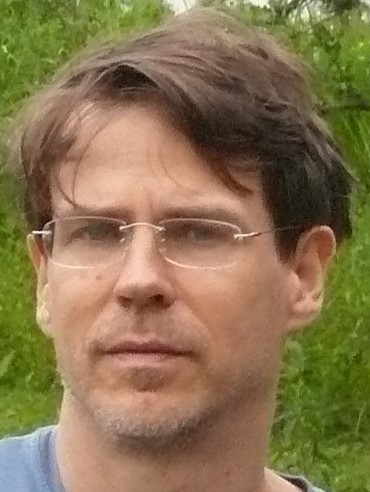
\includegraphics[scale=0.3,keepaspectratio]{images/fernando.jpg} 
  \end{flushright} 
   \end{column} %%% SINGULAR
 \end{columns}


\end{frame}


\subsubsection{Physics}

\begin{frame}{Academic Activities}

\begin{itemize}
  \item Wave equation in curved space-time.
  \item Gr\"obner bases.
  \item Pedagogical aspects of Special and General Relativity.
  \item Fractional calculus applied to viscoelastic problems.
  \item Research Groups at UDESC: COCA (Cognitive Computation) and Mathematical Physics.
\end{itemize}
\end{frame}

\subsubsection{Teaching Duties}

\begin{frame}{Teaching Activities}

\begin{itemize}
  \item Numerical Analysis.
  \item Complex Analysis.
  \item Vector Analysis.
  \item Ordinary Differential Equations.
  \item History of Mathematics.
  \item Distance education in mathematics (YouTube: Sasse)
\end{itemize}
\end{frame}

%%%%%%%%%%%%%%%%%%%%%%%%%%%%%%%%%%%%%%
\subsection{Claudio Cesar de Sá}

\begin{frame}{Claudio Cesar de Sá}

\begin{columns} %%% Começa o ambiente de Coluna
  \begin{column}{0.5\textwidth} %% 1a coluna
   \begin{itemize}
    \item Dr., Technological Institute of Aeronautics, 1997
    \item claudio.sa@udesc.br
    \item Departamento de Ciência da Computação, CCT- UDESC
    \item Research Group at UDESC: COCA 
    \end{itemize}
  \end{column}
   \begin{column}{0.5\textwidth}  %% 2a coluna --- SINGULAR
   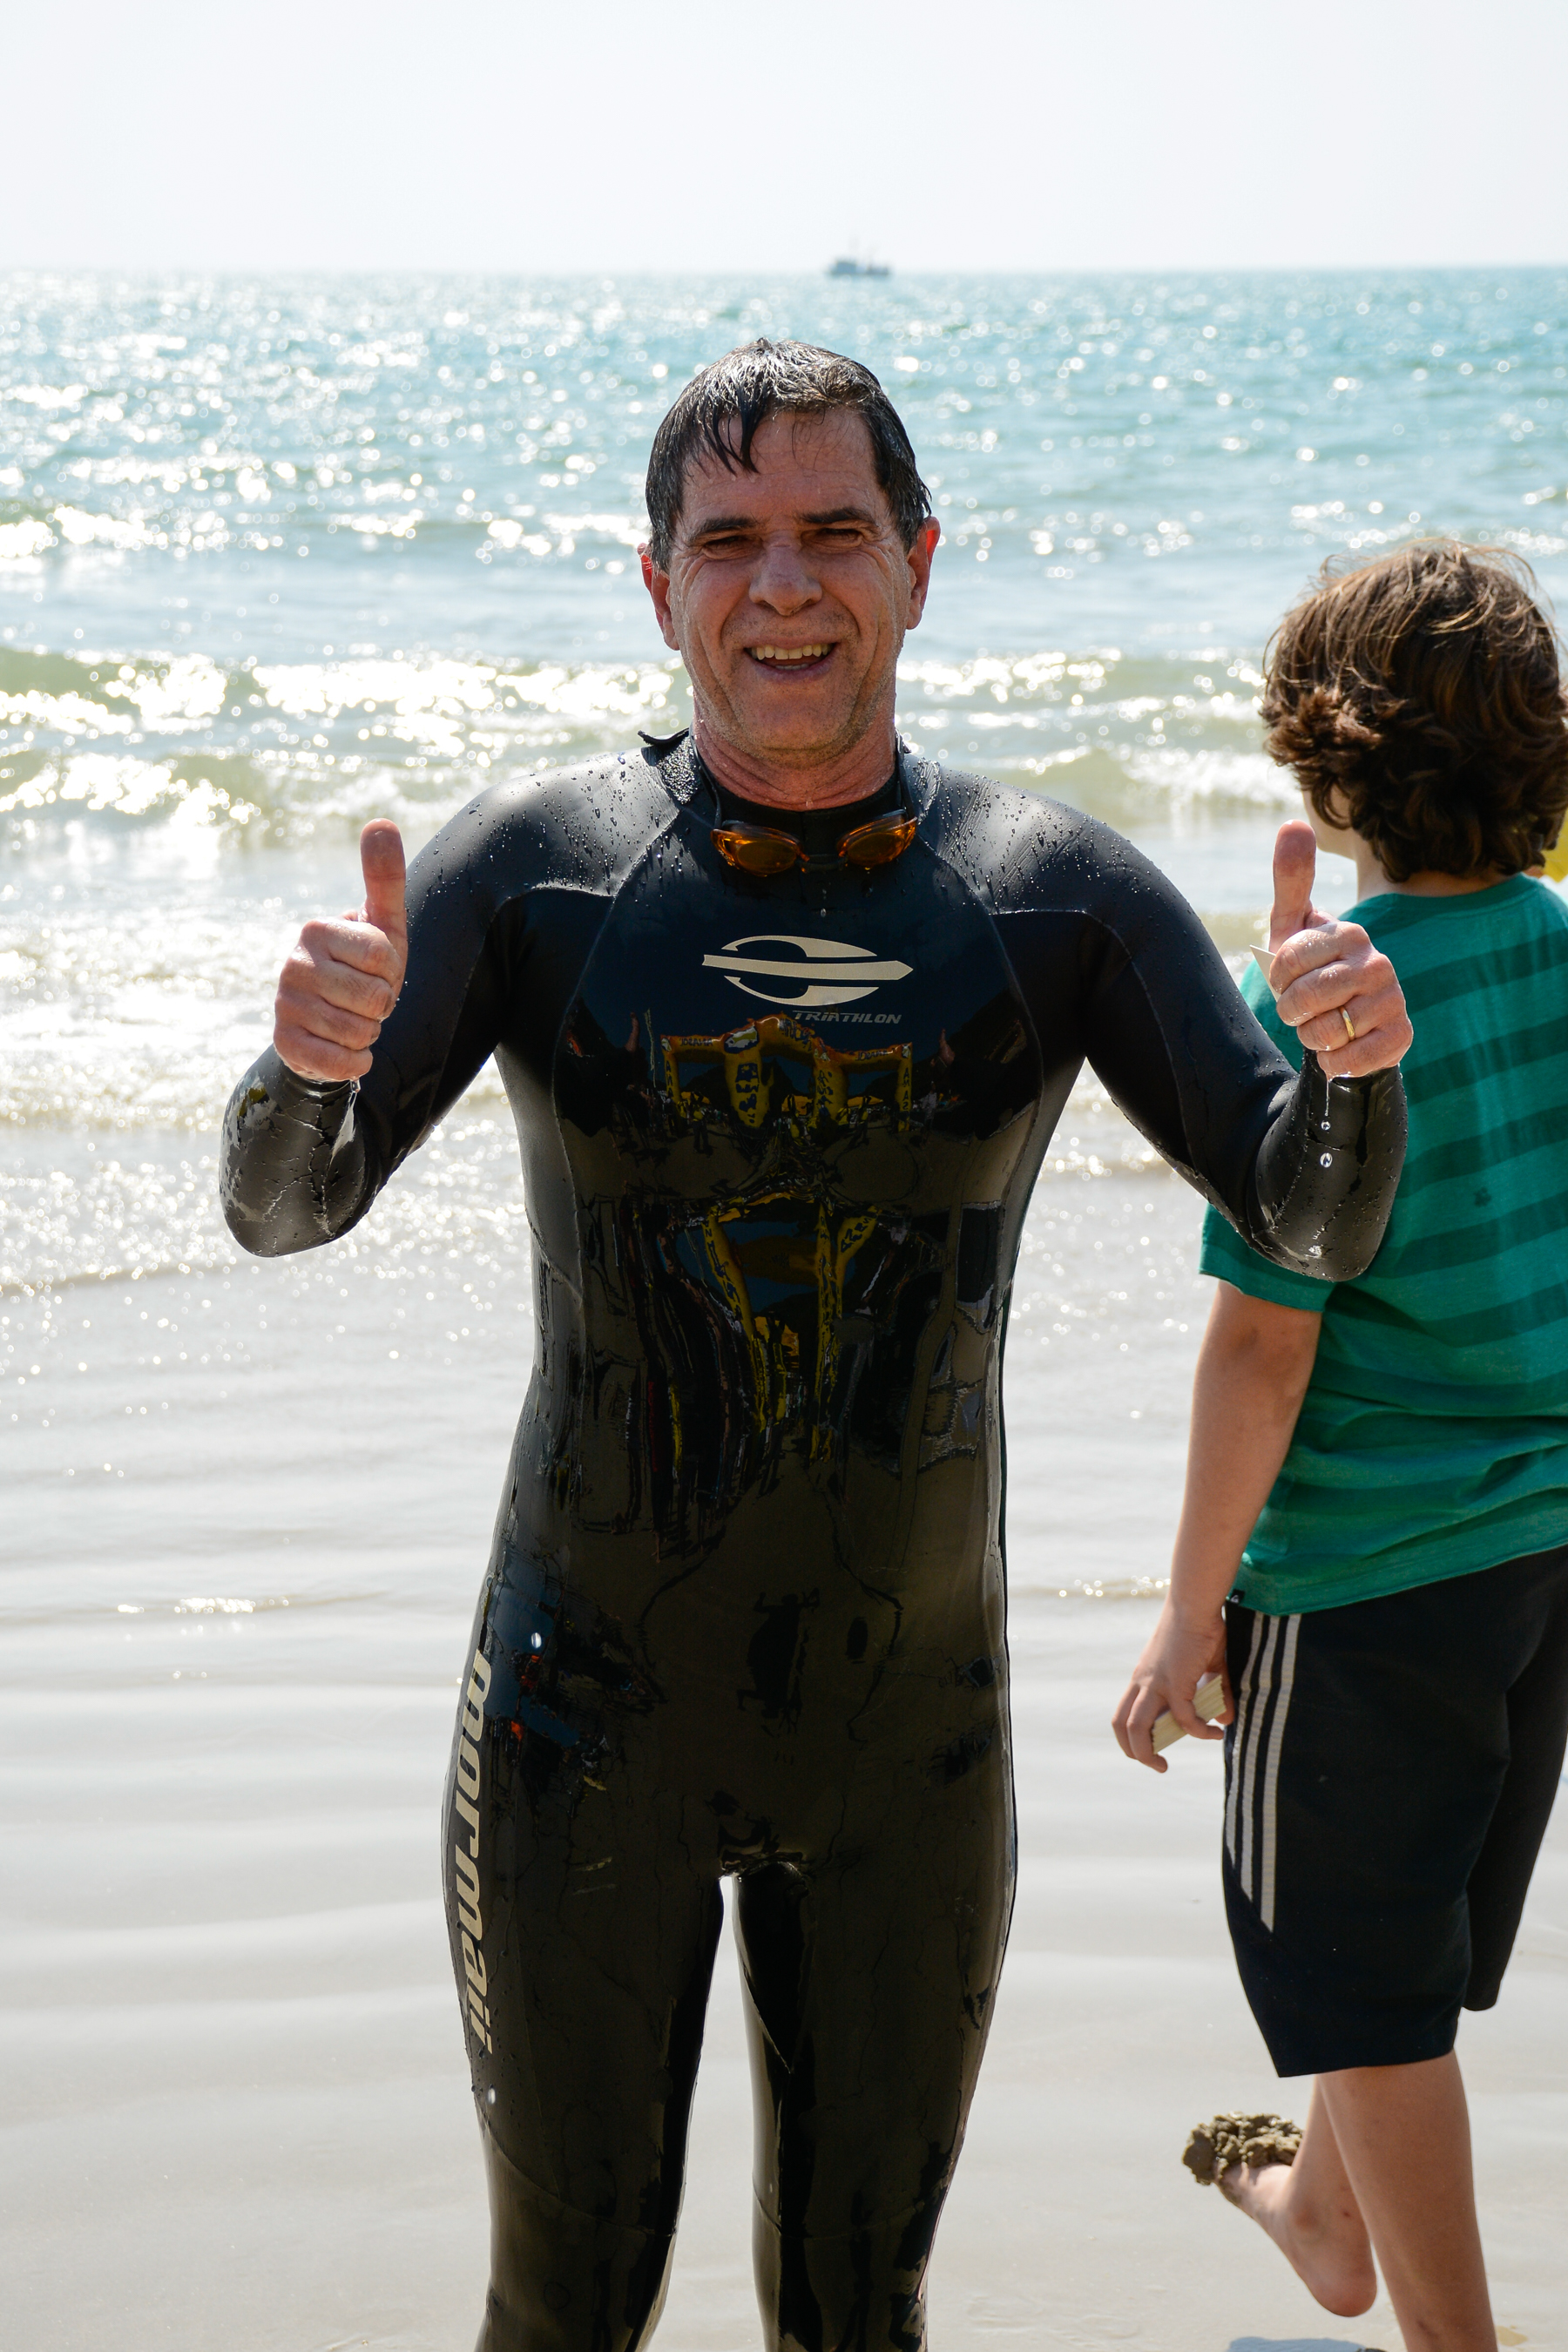
\includegraphics[scale=0.28,keepaspectratio]{images/maratona01.jpg}
  \end{column} %%% SINGULAR
 \end{columns}
 
%%%%%%%%%%%%%%%%%%%%%% 
\end{frame}


\subsubsection{Computing}
\begin{frame}{Academic Activities}

\begin{itemize}
  \item Artificial Intelligence $\rightarrow $ applied to solve real problems
  \item Combinatorial (Discrete) Optimization
  \item Modelling with Constraint Programming: PICAT and Minizinc
  \item Declarative Languages
  \item Free Hardware and Software 
\end{itemize}



\end{frame}

\subsubsection{Teaching Duties}
\begin{frame}{Teaching Activities}

\begin{itemize}
  \item Mathematical Logic
  \item Theory of Computation
  \item Formal Methods
  \item Foundations of Constraint Programming
  \item Programming Languages
 
\end{itemize}
\end{frame}

\subsubsection{Additional Activities}
\begin{frame}{Additional Activities}

\begin{itemize}
  \item Enrolled in Free Software Community
  \item General coordination: Contest Programming of ACM in UDESC
  \item Consulting of some enterprises: essentially courses
  \item Currently, developing an embedded system with free software for a {\em start-up}
\end{itemize}
\end{frame}




\subsubsection{Some Historical Projects}

\begin{frame}{Electrical Panels, Wires and Constraints}

\begin{columns} %%% Começa o ambiente de Coluna
  \begin{column}{0.5\textwidth} %% 1a coluna
  \begin{figure}[!ht]
    

   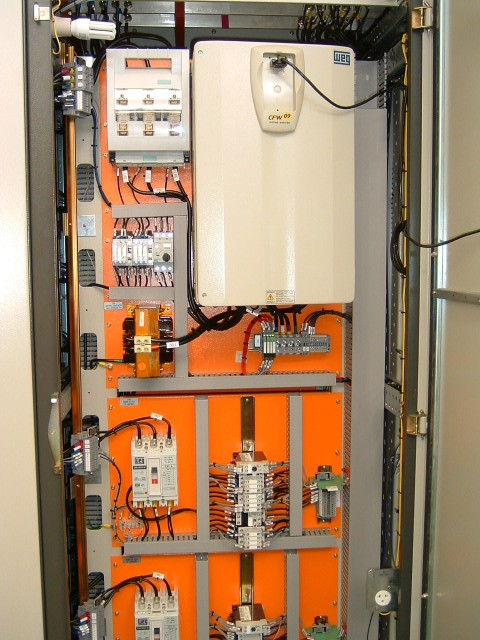
\includegraphics[scale=1.0,keepaspectratio]{images/painel.jpg}
   \caption{Real Panel}
     \end{figure}
  \end{column}
   \begin{column}{0.5\textwidth}  %% 2a coluna --- SINGULAR
     \begin{figure}[!ht]
   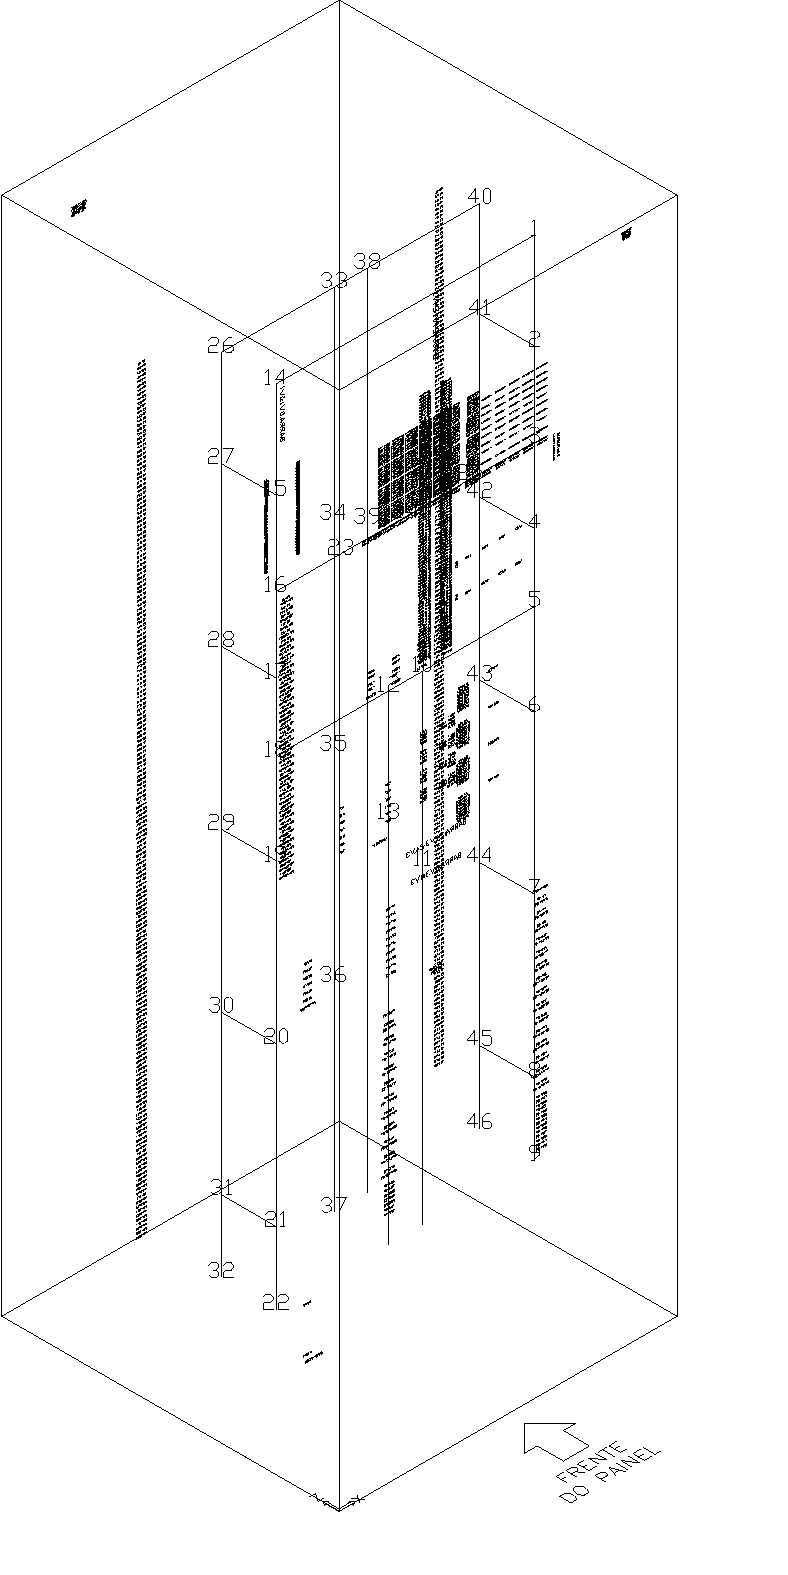
\includegraphics[scale=0.25,keepaspectratio]{images/painel_modelo.pdf}
   
      \caption{The panel and its complexity}
     \end{figure}
  \end{column} %%% SINGULAR
 \end{columns}
  

\end{frame}



\begin{frame}{Cellular Automata Applied in the Tumor Envolving}

\begin{columns} %%% Começa o ambiente de Coluna
  \begin{column}{0.5\textwidth} %% 1a coluna
  \begin{figure}[!ht]
   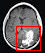
\includegraphics[scale=3.0,keepaspectratio]{images/ac_EntradaExemplo.png}
   \caption{The real initial state}
     \end{figure}
  \end{column}
   \begin{column}{1.0\textwidth}  %% 2a coluna --- SINGULAR
     \begin{figure}[!ht]
   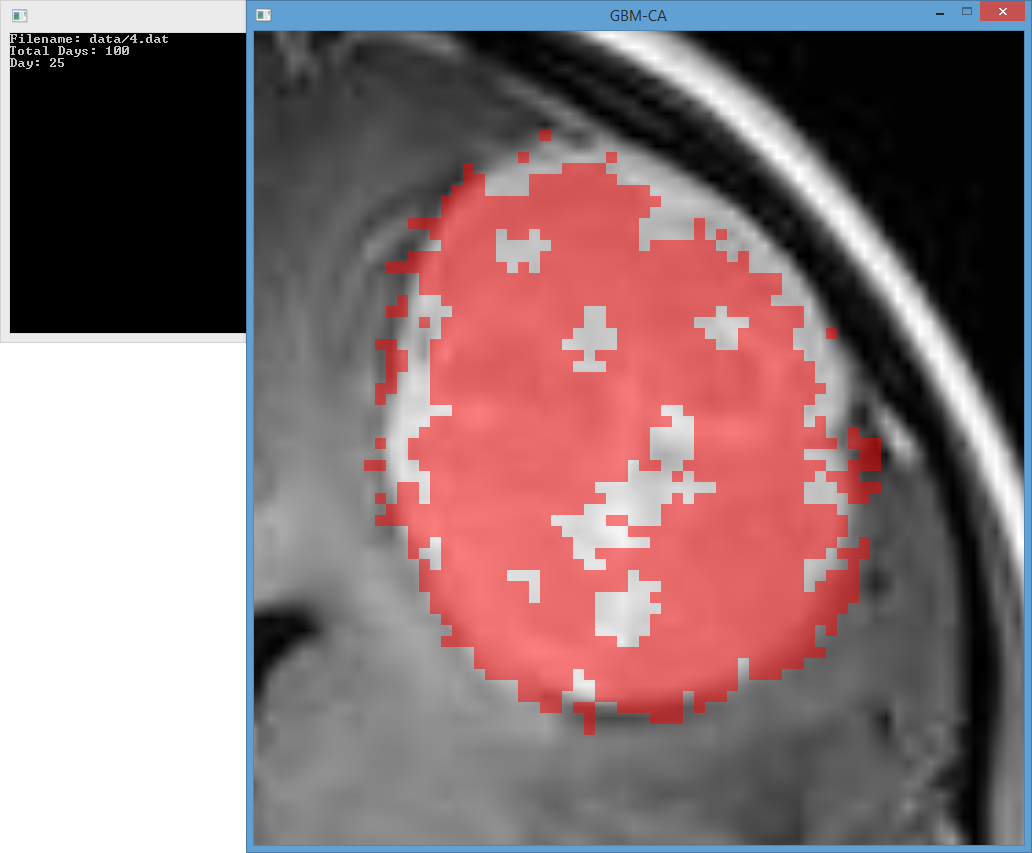
\includegraphics[scale=0.2,keepaspectratio]{images/ac_SimulacaoExemplo.png}
   
      \caption{The simulation}
     \end{figure}
  \end{column} %%% SINGULAR
 \end{columns}
  

\end{frame}



%%%%%%%%%%%%%%%%%%%%%%%%%%%%%%%%%%%%%%%%%%%%%%%%
%%%%%%%%%%%%%%%%%%%%%%%%%%%%%%%%%%%%%%%%%%%%%%%%
\subsection{Rafael Stubs Parpinelli}
\begin{frame}{Rafael Stubs Parpinelli}

 \begin{columns}
 \begin{column}{0.5\textwidth} 
  \begin{itemize}
  \item Dr., Federal Technological University of Paran\'a, 2013
  \item rafael.parpinelli@udesc.br
  \item Department of Computer Science, CCT - UDESC
  \item Graduate Program in Applied Computation, CCT - UDESC
  \item Research Groups at UDESC: COCA and Group of Control and Systems (Department of Electrical Engineering).
\end{itemize}

 \end{column}
 
   \begin{column}{0.5\textwidth}  %% 2a coluna --- SINGULAR
  \begin{flushright}
   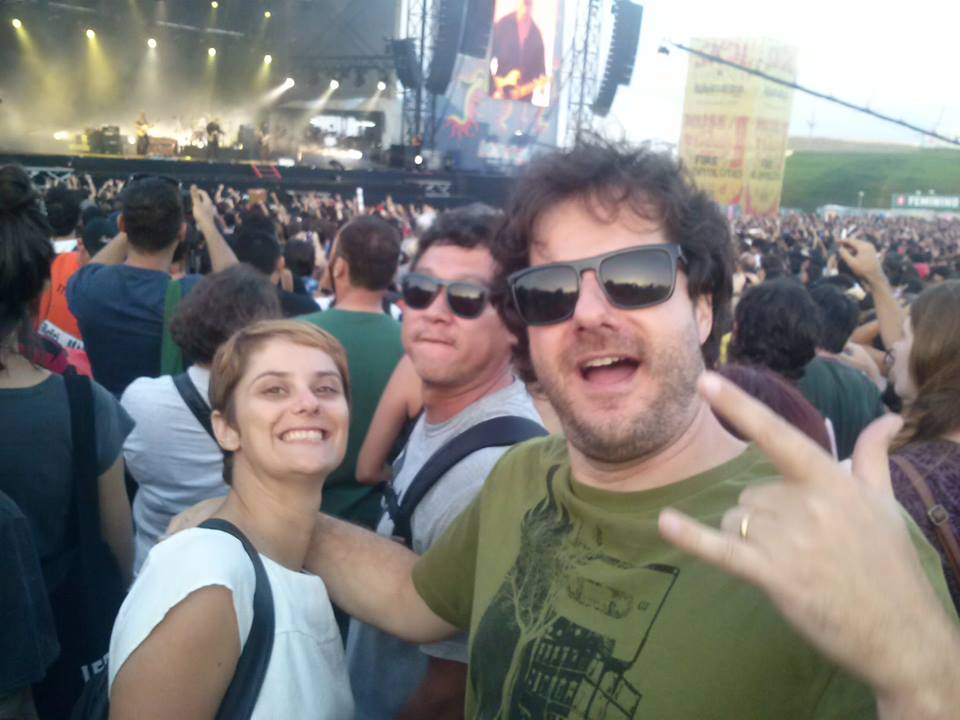
\includegraphics[scale=0.18,keepaspectratio]{images/rafael.jpg} 
  \end{flushright} 
   \end{column} %%% SINGULAR
 \end{columns}
 
\end{frame}
 
\subsubsection{Computing}

\begin{frame}{Academic Activities}

\begin{itemize}
  \item Head of COCA (together with Prof. Claudio)
  \item Research Projects concerning the application of Computational Intelligence in: 
  \begin{itemize}
   \item Optimization of Complex Problems.
   \item Data Mining.
   \item Bioinformatics.
   \item Development of new Bio-inspired algorithms.
  \end{itemize}
  \item Tutoring: 2 Undergraduate Students, 2 Scientific Initiation Students, 3 Graduate Students (M.Sc.).
  \item Reviewer of IEEE Transactions on Evolutionary Computation, IEEE Transactions on Systems, Man and Cybernetics, and others.
  \item Program Committee member of several events.
\end{itemize}
\end{frame}

\subsubsection{Teaching Duties}

\begin{frame}{Teaching Activities}

\begin{itemize}
  \item Evolutionary Computation.
  \item Swarm Intelligence.
  \item Artificial Intelligence.
  \item Natural Computing.
  \item Discrete Mathematics.
\end{itemize}
\end{frame}
%%%%%%%%%%%%%%%%%%%%%%%%%%%%%%%%%%%%%%%%%%%%%%%%
%%%%%%%%%%%%%%%%%%%%%%%%%%%%%%%%%%%%%%%%%%%%%%%%
\subsection{Rogério Eduardo da Silva}
\begin{frame}{Rogério Eduardo da Silva}


\begin{columns}
\begin{column}{0.5\textwidth} 
\begin{itemize}
  \item Ph.D, University of Minho/Portugal, 2014
  \item rogerio.silva@udesc.br and \url{http://www.rogerioesilva.net/}
  \item Department of Computer Science, CCT - UDESC
  \item Research Groups at UDESC: COCA 
\end{itemize}
 \end{column}

   \begin{column}{0.5\textwidth}  %% 2a coluna --- SINGULAR
  \begin{flushright}
   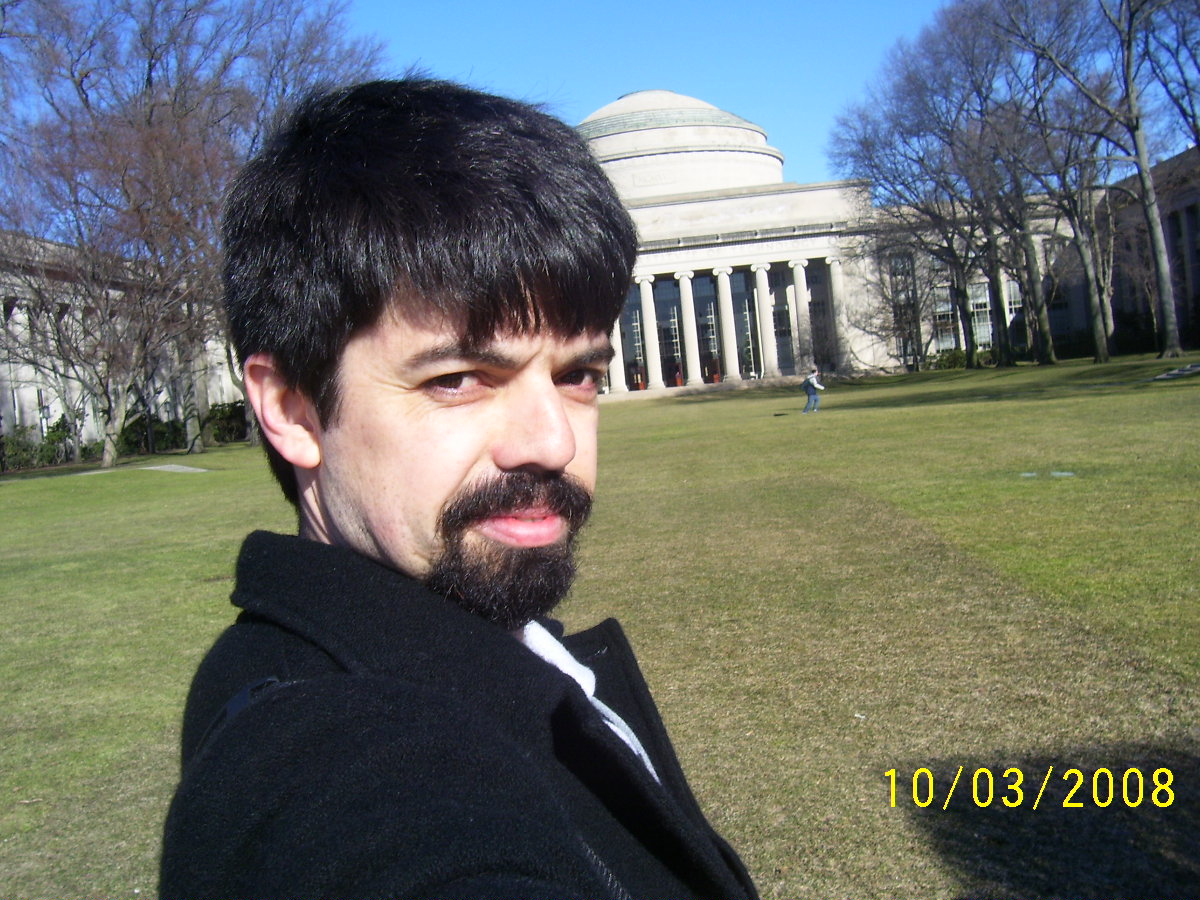
\includegraphics[scale=0.15,keepaspectratio]{images/mit-roger.jpg} 
  \end{flushright} 
   \end{column} %%% SINGULAR
 \end{columns}


\end{frame}


\subsubsection{Computing}

\begin{frame}{Academic Activities}

\begin{itemize}
  \item Researches Multi-Agents Systems applied to Interactive Digital Storytelling systems that consider: 
  \begin{itemize}
	 \item Knowledge Representation and Reasoning
   \item Computational Psychology
   \item Affective Computing
   \item Autonomous Agents
   \item Virtual Humans
  \end{itemize}
  \item Tutoring: 1 Undergraduate Student, 3 Scientific Initiation Students
	\item Check it out! \url{http://drama.musa.cc/}
\end{itemize}
\end{frame}

\subsubsection{Teaching Duties}

\begin{frame}{Teaching Activities}

\begin{itemize}
  \item Mathematical Logic
  \item Multi-Agents Systems
  \item Data Structures II
\end{itemize}
\end{frame}

%%%%%%%%%%%%%%%%%%%%%%%%%%%%%%%%%%%%%%%%%%%%%%%%

\subsubsection{This Presentation}

\begin{frame}{Our site and this presentation:}


  
  \begin{center}
   
\includegraphics[scale=0.6,keepaspectratio]{images/simpsons.jpg} 
  \end{center} 
  

\begin{itemize}
  \item \url{http://www.joinville.udesc.br/coca/} $\rightarrow $ Members

  \item Thank you so much!
\end{itemize}




\end{frame}


\end{document}
